\documentclass{article}
\usepackage{tikz}

\newcommand*{\xMin}{0}%
\newcommand*{\xMax}{23}%
\newcommand*{\yMin}{0}%
\newcommand*{\yMax}{6}%

\begin{document}
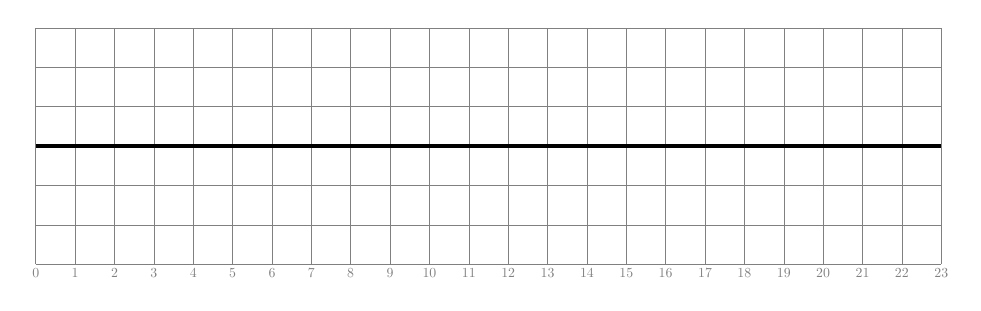
\begin{tikzpicture}[thick,scale=0.5, every node/.style={scale=0.5}]
    \foreach \i in {\xMin,...,\xMax} {
        \draw [very thin,gray] (\i,\yMin) -- (\i,\yMax) node [below] at (\i,\yMin) {$\i$};
    }
    \foreach \i in {\yMin,...,\yMax} {
%        \draw [very thin,gray] (\xMin,\i) -- (\xMax,\i) node [left] at (\xMin,\i) {$\i$};
        \draw [very thin,gray] (\xMin,\i) -- (\xMax,\i);

    }

% \draw [step=1.0,blue, very thick] (0.5,0.5) grid (5.5,4.5);
% \draw [very thick, brown, step=1.0cm,xshift=-0.5cm, yshift=-0.5cm] (0.5,0.5) grid +(5.5,4.5);

\draw [very thick, black] (0,3) -- (\xMax, 3);

\end{tikzpicture}
\end{document}